\newacronym{rnd}{R\&D}{Research and Development}
\newacronym{etl}{ETL}{Extract, Transform, Load}
\newacronym{rdbms}{RDBMS}{Relational Database Management System}
\newacronym{pbe}{PBE}{Programming by Example}
\newacronym{lpbd}{L/PBD}{Learning/Programming by Demonstration}
\newacronym{gui}{GUI}{Graphical User Interface}
\newacronym{dsl}{DSL}{Domain-Specific Language}
\newacronym{ide}{IDE}{Integrated Development Environment}
\newacronym{rdf}{RDF}{Resource Description Framework}
\newacronym{rcp}{RCP}{Rich Client Platform}
\newacronym{cli}{CLI}{Command Line Interface}
\newacronym{repl}{REPL}{Read--Eval--Print Loop}

\newglossaryentry{datawarehousing}
{
  name={data warehousing},
  description={is a classic approach to analytical reporting based on data marts mostly periodically fed from multiple sources}
}

\newglossaryentry{semanticweb}
{
  name={semantic web},
  description={is a buzzword term commonly subsuming approaches and technologies supporting the notion of making the mainly text-based, unstructured data on the \textsc{WWW} more accessible by enriching it with machine-readable semantics}
}


The report or review contained in this chapter focuses on summarizing and comparing approaches\index{approach}, techniques, and related work within the field which can generally be subsumed by the term \emph{``\textbf{\gls{datawrangling}}''} with an emphasis on \textbf{visual-interactive\index{visual-interactive} support}.
This is a relatively young field of interdisciplinary \gls{rnd}.
It is basically about the process of making any data useful for analysis\index{analysis}.
This reviewing report is mainly geared towards offering an overview of the topic in order to comprehensively show differences of existing approaches\index{approach} as well as commonalities shared between them.
Furthermore, special attention is paid to setting it all into the historic evolutionary context of the field.
In the end, we can see that there is still some need for exploration and improvements here, particularly regarding visual-interactive\index{visual-interactive} components and the support for time-oriented\index{time-oriented} data.

This chapter gives a brief overview of related work, i.e., its scientific underpinnings, followed by a walkthrough of different concrete approaches\index{approach}, techniques, and related tools.

\section{Literature Study}

Generally, \cite{Kandel2011a} was used as a point of origin to find other relevant references.
Then, going through the list of references of these papers, relevance was determined via personal evaluation.
Plus, we scanned the reference lists of thus relevant papers.

Moreover, we searched the archives of topic-related journals (i.e., \emph{Information Visualization Journal} and \emph{ACM Journal of Data and Information Quality}) as well as scientific, electronic databases (\emph{ACM Digital Library}, \emph{IEEE Xplore}, and also \emph{Google Scholar}) and proceedings of relevant conferences (\emph{International Conference on Information Visualization}, \emph{IEEE Conference on Visual Analytics}, \emph{ACM SIGCHI Conference on Human Factors in Computing Systems}, etc.).

Our search terms included \emph{``data wrangling''}, \emph{``data cleansing''}, and variations of these phrases.
\emph{Mendeley}\footnote{\textcolor{blue}{\href{https://www.mendeley.com/}{www.mendeley.com}}} was used as a tool to conveniently keep track of references and organize our bibliography.

We want to span a comprehensive overview of different approaches\index{approach} to the topic, focusing on the evolution over time here.

Basics of the field are laid out in \cite{Dasu2003}, mainly relating to \textbf{\gls{etl}} processes as classically known from \textbf{\gls{datawarehousing}}.
General theoretical foundation of transforming\index{transformation} large amounts of data interactively can be found in \cite{Dasu2002} and more recently \cite{Hellerstein2008}.
While the former can be seen as a valuable general resource on the topic with focus on \gls{rdbms}, the latter is especially interesting as a contemporary specimen spanning a rather wide range of scientific ground.
In particular, \cite{Hellerstein2008} explains the statistics\index{statistics} theory backing things like outlier detection and puts it into applied context, e.g., via showing corresponding \textsc{SQL} queries implementing this.
In the end, there is a section focusing on actual interface design\index{design} principles regarding the topic of exploratory quantitative data cleaning.
To complete the selection here, basic algorithmic theory of interactive schema mapping and its application is covered, e.g., by \cite{Chiticariu2008}.
The matter is relevant in this regard as it is concerned with interactively (and usually visually) transforming\index{transformation} data (schemas in this case) as well.

More recently, another interesting field of research commonly referred to as \emph{``Learning by \textbf{Example}''} or more concretely \emph{``\textbf{\gls{pbe}}''} has emerged.
Traditionally, there has been the approach\index{approach} of \emph{``\gls{lpbd}''} which requires users to specify start, end, as well as intermediate states of the respective task at hand to be automated.
See \cite{Gulwani2010} for an overview survey of the foundations of this research area, more generally called \emph{``\textbf{program synthesis}''}.
Based on the work of \cite{Gulwani2011}, Microsoft Excel 2013 is incorporating such concepts (i.e., particularly applied \gls{pbe}) into commercial software for end-users.
That is, users can show the application which parts of the data they are interested in by simply marking or highlighting examples and an underlying engine infers corresponding wrangling\index{wrangle} transformations\index{transformation} from that -- without requiring demonstration of any intermediary steps.


\section{Analysis}

This section presents more concrete approaches\index{approach} and examples, historically aligned, followed by a comparison and outlook for our prototype\index{prototype}.

\subsection{Potter's Wheel: A Pioneer}

A system pioneering this area is called \emph{Potter's Wheel}, ~\cite{Raman2001a}. It offers a spreadsheet-like \gls{gui} for interactively specifying and executing data transformations\index{transformation} (see Figure~\ref{fig:potters-wheel-screenshot} for a screenshot, as presented in the paper).

This can be done either via \emph{\gls{lpbd}} (i.e., the user ``shows'' what he wants to achieve and the system tries to infer actions from this) or somewhat direct manipulation via corresponding menus.
Yet, among other things, it does not support ``fill'' transform\index{transformation} operations (that is, automatically filling certain fields with certain data, batch-wise).
Plus, naturally, its usability is not up to modern standards.

On the \textbf{pro} arguments side: important step into the direction of visual-interactively\index{visual-interactive} supporting users in \gls{datawrangling} tasks.

On the \textbf{con} arguments side: as stated above, raw (also due to its pioneering status) implementation with room for improvements and there is no real charting support.

\begin{figure}[h]
  \centering
  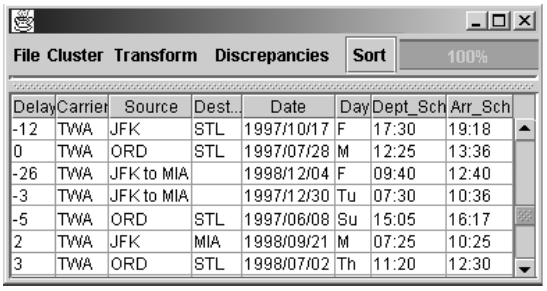
\includegraphics[width=0.7\textwidth]{figures/state-of-the-art/potters-wheel}
  \caption{Showing Potter's Wheel spreadsheet-like \gls{gui} approach\index{approach}. Transform operations are accessible via menu bar~\cite{Raman2001a}.}
  \label{fig:potters-wheel-screenshot}
\end{figure}


\subsection{PADS: A Domain-Specific Language Approach}

The system of \cite{Fisher2005} approaches\index{approach} the topic of transforming\index{transformation} large amounts of semi-structured data via a descriptive \textbf{\gls{dsl}}.
Consequently, it is lacking a visual-interactive\index{visual-interactive} component altogether and taken into consideration here for the sake of completeness and demonstrating a different solution view.
Users describe the data that is to be transformed\index{transformation} in the \gls{dsl}.
Then the \emph{PADS} compiler allows for generating (\textsc{C}-based) parser libraries and built-upon tools for further processing of such data.
The project was conducted at \emph{AT\&T} and focuses on specific data transformation\index{transformation} requirements of the company at that time.
Target output data formats are in particular \textsc{XML} and ones for loading the data into \gls{rdbms}es (i.e., \textsc{SQL}).
Mainly supported input formats are of \textsc{ASCII} (log files), binary (legacy networking protocols), and Cobol kind.
\\\\
Here is some exemplary web server access logs input data as shown in the paper:

{\tiny
  \begin{verbatim}
    207.136.97.49 - - [15/Oct/1997:18:46:51 -0700] "GET /tk/p.txt HTTP/1.0" 200 30
    tj62.aol.com - - [16/Oct/1997:14:32:22 -0700] "POST /scpt/dd@grp.org/confirm HTTP/1.0" 200 941
  \end{verbatim}
}

A \textbf{pro} argument for this approach\index{approach} is that the \gls{dsl} is relatively concise and easily graspable due to its declarative nature.
Furthermore, it frees its users from manually writing parsers and constructive tools as these are generated from the \gls{dsl} definitions of a concrete data format to work with.
Finally, the quality and range of tools can be improved and extended in a convenient way being quite independent from the generated parsers.

If we wanted to find a \textbf{con} argument here it could be that while being useful and a general step forward at the time of development, we believe that there are probably better ways to support certain kinds of end-users in these tasks, namely of the visual-interactive\index{visual-interactive} kind which we want to evaluate with this thesis after all.


\subsection{Microsoft BizTalk Schema Mapper Research}

In the approach\index{approach} of ~\cite{Robertson2005}, Microsoft's \emph{BizTalk} schema mapper application is attempted to be improved.
Main use case being visual and interactive support of mapping two differing \textsc{XML} schemas.
Moreover, the schemas are of considerable big size (i.e., thousands of elements in each schema) to be not processable in a usable way within the traditional \gls{ui}.
That is, too many connections between the schemas are shown in a too complex way to be useful.
To improve the \gls{ui} some \gls{infovis} techniques are applied (Figure~\ref{fig:biztalk-research-screenshot} presents a screenshot showing this).

As described by the authors, these techniques are:

\begin{itemize}
  \item \textbf{Highlight propagation:} \\(de-)emphasizing areas of interest within the mapping \gls{ui}
  \item \textbf{Auto-scrolling:} \\automatically scrolling to selected items (comparable to \glslink{ide}{IDEs}) etc.
  \item \textbf{Coalescing trees:} \\somewhat relating to highlight propagation hiding irrelevant nodes
  \item \textbf{Multi-select:} \\reasonable support for multi-selection of nodes concerted with general visualization
  \item \textbf{Incremental search:} live search results updating the \gls{ui} while typing
  \item \textbf{Bendable links:} enabling the user to see connections when actually overlayed
  \item \textbf{Focus on linked elements:} improved default behavior of up/down keys usage
\end{itemize}

The results are evaluated via a user study and have proven to be useful which can be seen as a \textbf{pro} argument here as well.

There is little to mention on the \textbf{con} side regarding the approach\index{approach} of ~\cite{Robertson2005} as it overall demonstrates an advancement in the area of interactive schema mapping.

\begin{figure}[h]
  \centering
  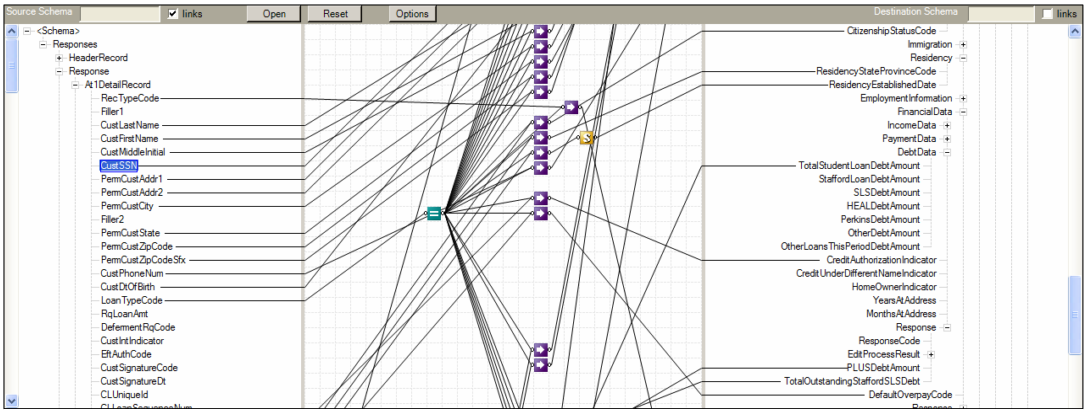
\includegraphics[width=1.0\textwidth]{figures/state-of-the-art/biztalk-research}
  \caption{BizTalk research GUI demonstrating some applied InfoVis techniques. On each vertical side of the visible pane, elements of a respective schema are represented by a tree-like structure. Mappings between them are visualized as arcs. Center nodes are used for displaying more complex (m:n-like) mappings~\cite{Robertson2005}.}
  \label{fig:biztalk-research-screenshot}
\end{figure}


\subsection{Clio: From Research Prototype to Industrial Tool}

In ~\cite{Haas2005} the authors outline the evolution of an IBM research prototype\index{prototype} to an industrial-strength tool.
\emph{Clio} is an application for descriptive specification of schema mappings.
It is mainly targeted towards \textsc{XML} and relational schemas (see Figure~\ref{fig:clio-screenshot}).
So, in this respect it is quite similar both by field and application to the aforementioned Microsoft \emph{``BizTalk''} schema mapper product, adding \gls{rdbms}/\textsc{SQL} mapping to the mix.
Mappings are represented by an abstract query graph allowing for translation of data transformations\index{transformation} into specific query languages.
This is what makes it interesting and distinguishing, again, when compared with Microsoft's \emph{BizTalk} schema mapping application.

Finally, the paper focuses on revisiting the architecture\index{architecture} and algorithms behind the software and then explains issues and solutions on the way to applying industrial usage.
Consequently, it is a useful real-world example of transferring science in practice.

\begin{figure}[h]
  \centering
  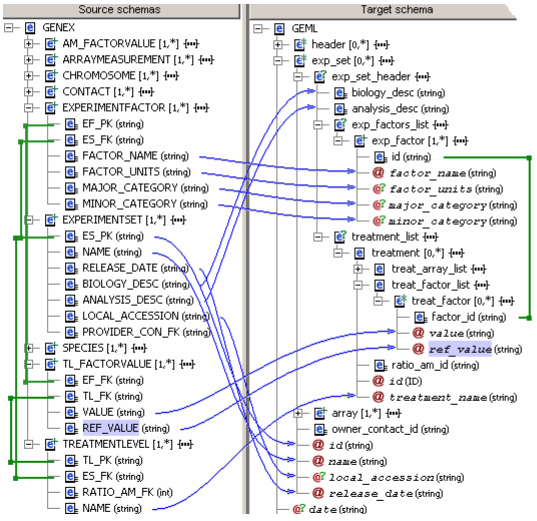
\includegraphics[width=0.66\textwidth]{figures/state-of-the-art/clio-grown-up}
  \caption{Clio GUI, also showing similarities with the MS BizTalk one. Consequentially, again, data schemas (this time from relational DBs, though) on the left and right-hand sides with mappings as arrowed lines~\cite{Haas2005}.}
  \label{fig:clio-screenshot}
\end{figure}


\subsection{Potluck: A Semantic Web Approach}

The research prototype\index{prototype} in \cite{Huynh2007} focuses on making heterogeneous \textbf{\emph{\gls{semanticweb}}} data accessible to casual users.
It provides a web interface for visual and interactive wrangling\index{wrangle} of data mainly relating to \gls{rdf}.
An interesting feature is allowing users to tag and visualize data with physical locations via a map view (see Figure~\ref{fig:potluck-map-screenshot}).
What is also interesting in this approach\index{approach} is its demonstration of increased interest respectively shift towards web technologies at that time.
Furthermore, it delivers some kind of preview how far web-based approaches\index{approach} would go in this area.
Plus, it illustrates the general trend in the direction of casual end-user applications (enabling non-expert users to operate actually complex tasks).

\begin{figure}[h]
  \centering
  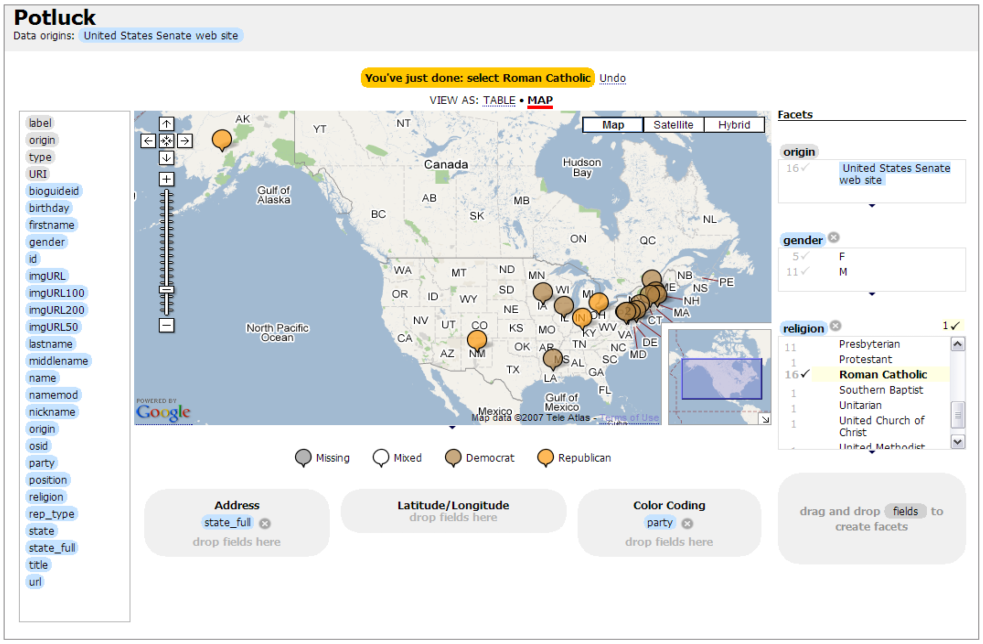
\includegraphics[width=1.0\textwidth]{figures/state-of-the-art/potluck-map-view}
  \caption{Potluck map view which can be seen as a back then innovative visualization in the field. Data is displayed geospatially~\cite{Huynh2007}.}
  \label{fig:potluck-map-screenshot}
\end{figure}

\newpage


\subsection{\gls{rnd} Veterans: DataWrangler \& OpenRefine}

The two systems that can be the seen to have set the benchmark in this space are:

\begin{enumerate}
  \item \textbf{\emph{DataWrangler}} (\emph{Stanford Visualization Group} research project\footnote{\textcolor{blue}{\href{http://vis.stanford.edu/wrangler/}{vis.stanford.edu/wrangler/}}})~\cite{Kandel2011a}
  \item \textbf{\emph{OpenRefine}} (open-sourced\footnote{\textcolor{blue}{\href{https://github.com/OpenRefine/OpenRefine}{github.com/OpenRefine/OpenRefine}}} product\footnote{\textcolor{blue}{\href{http://openrefine.org/}{openrefine.org}}} f.k.a. \emph{Google Refine} and \emph{Freebase Gridworks})
\end{enumerate}


\subsubsection{DataWrangler}

\emph{DataWrangler}, cf. Kandel et al. in~\cite{Kandel2011a}, is a web-browser-based application oriented towards a visually interactive approach\index{approach} (see Figure~\ref{fig:data-wrangler-screenshot}).
It contains an inference engine suggesting transforms\index{transformation}, plus, data cleaning sessions can be exported and reused as scripts.
The creators of the project meanwhile moved on to make a commercial product out of it, called \emph{Trifacta Wrangler}\footnote{\textcolor{blue}{\href{https://www.trifacta.com/products/wrangler/}{www.trifacta.com/products/wrangler/}}}.

One thing which is less supported by \emph{Wrangler} is full-control direct manipulation of data.
That is, it is more geared towards \gls{lpbd} than to deliberately changing the content of single values via direct input.

In addition to that, the \gls{ui} is limited which can also be ascribed to the web-based nature of the tool.
Things like not truly responsively, and richly interactive \gls{ux}, especially when the amounts of data that are to be wrangled\index{wrangle} grow.

DataWrangler was evaluated via a user study and has shown to improve productivity of \gls{datawrangling} tasks considerably.

Biggest \textbf{pro} arguments of the approach\index{approach}:

\begin{itemize}
  \item Interactively inferred suggested transforms\index{transformation}
  \item Rich collection of transforms\index{transformation} to be applied
  \item Shows the potential of pursuing the visual-interactive\index{visual-interactive} path
\end{itemize}

Main \textbf{con} argument is performance-wise constrained usefulness of the tool and its generally improvable \gls{ux}.
Also, no real charting support available, yet.

\begin{figure}[h]
  \centering
  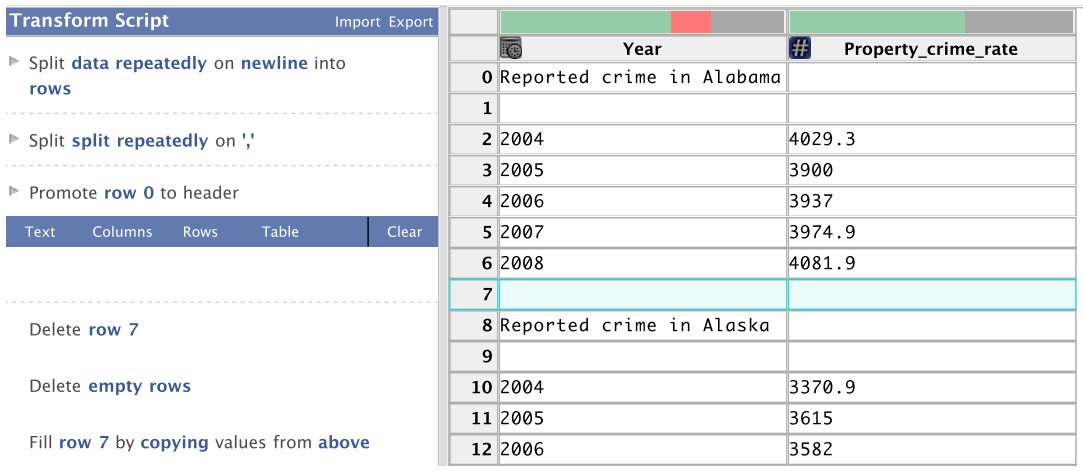
\includegraphics[width=1.0\textwidth]{figures/state-of-the-art/data-wrangler}
  \caption{DataWrangler \gls{ui} as a state of the art shaping, innovative approach\index{approach}. Data transform history and related suggestions are located on the left, tabular interaction pane on the right~\cite{Kandel2011a}.}
  \label{fig:data-wrangler-screenshot}
\end{figure}


\subsubsection{OpenRefine}

\emph{OpenRefine} is a browser-based application as well (but running locally on the user's machine, also due to data protection respectively privacy reasons).
It allows for direct manipulation of data (see Figure~\ref{fig:open-refine-screenshot}), yet, it supports less interaction-driven transform\index{transformation} operations than DataWrangler (which infers appropriate transformation\index{transformation} suggestions from solely pointing the cursor to data in a certain way).

A nice feature is its visual statistical\index{statistics} analytics of data distribution via histograms etc. ($\rightarrow$ \textbf{pro} argument).
But, on the \textbf{con} side, it generally lacks some data transformation\index{transformation} operations which are supported by DataWrangler (particularly reshaping-related, like un/folding -- extracting/merging specific parts of data within a column into/from additional ones).

\begin{figure}[h]
  \centering
  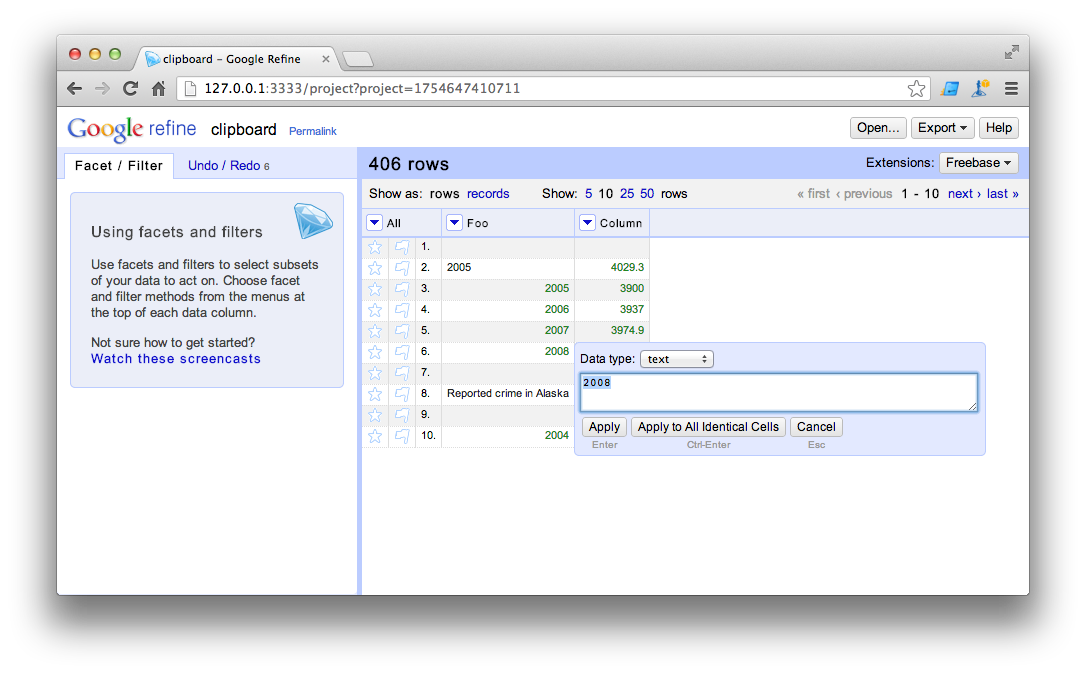
\includegraphics[width=1.0\textwidth]{figures/state-of-the-art/google-refine}
  \caption{Google/OpenRefine \gls{ui} in action, also offering direct manipulation of data. Again, as in DataWrangler, tabular respectively spreadsheet-like interface.}
  \label{fig:open-refine-screenshot}
\end{figure}


\subsection{Temporal Research: On Time Series Data}

The research prototype\index{prototype} in~\cite{Bernard2012} focuses specifically on time-series-based data.
It is tailored for joint usage of a domain and a \gls{datamining} expert.
Technically, a preprocessing pipeline is visual-interactively\index{visual-interactive} created and incrementally adjusted via the tool (see Figure~\ref{fig:time-series-research-screenshot}).

What is interesting here is the application of the domain on time series data.
Moreover, its pipeline-oriented workflow \gls{ui}, offering various statistical\index{statistics} visualizations, is a well-designed\index{design} asset.
Finally, the approach\index{approach} is evaluated by applying it to a case study delivering results proving it useful in its context.


\subsection{The Industry: Talend Open Studio}

Within the industry a well-known collection of enterprise tools is \emph{Talend Open Studio}\footnote{\textcolor{blue}{\href{https://www.talendforge.org/}{www.talendforge.org}}}.
This is an open source software suite with commercial support offerings.
Architecturally\index{architecture}, it is based on \emph{\textbf{Eclipse}} \gls{rcp}.
The product which can be used for \gls{datawrangling} is \emph{Talend Data Quality}\footnote{\textcolor{blue}{\href{https://www.talend.com/products/data-quality/}{www.talend.com/products/data-quality/}}} (see Figure~\ref{fig:talend-open-studio-screenshot} for its \gls{gui}).
It allows for interactive specification and execution of data transformations\index{transformation} with \textbf{visual charting aid}.
I.e., data at hand is visualized via meaningful charts while interactively manipulating it.


\subsection{An Innovative Approach\index{approach}: Kibana Timelion}

\emph{Kibana} is a product by the company \emph{Elastic} which is mainly geared towards visualizing data of their other product \emph{Elasticsearch} in an interactive fashion with charts.
As sort of a research project \emph{Timelion} was born (see \cite{web:Timelion} and Figure~\ref{fig:kibana-timelion}).
It allows for interactive exploration and transformation\index{transformation} of time series data with a programmatic, mathematical \gls{dsl} via a \gls{cli}.
Commands trigger chart visualizations accordingly.
The way these interaction methods are combined is rather unseen before.

Another Elastic product worth mentioning in our context is called \emph{Logstash}\footnote{\textcolor{blue}{\href{https://www.elastic.co/products/logstash}{www.elastic.co/products/logstash}}}.
This is basically a universal data processing engine with transformation\index{transformation} capabilities, historically focused on log event data, mainly driven by filter expressions written in \emph{Ruby}-like syntax.

\begin{figure}[h]
  \centering
  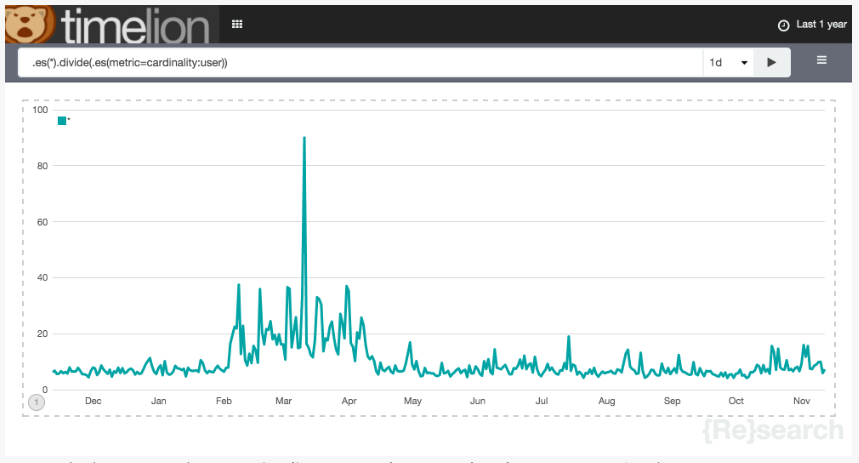
\includegraphics[width=1.0\textwidth]{figures/state-of-the-art/kibana-timelion}
  \caption{Kibana Timelion as an innovative approach to visual-interactively\index{visual-interactive} exploring and transforming time series data~\cite{web:Timelion}.}
  \label{fig:kibana-timelion}
\end{figure}


\subsection{Modern Data Science: Jupyter Notebooks}

\Gls{datascience} nowadays is commonly pursued with \emph{Jupyter Notebooks}\footnote{\textcolor{blue}{\href{https://jupyter.org/}{jupyter.org}}}.

These interactive notebooks are powered by a web-based application, often running locally and connecting to remote data sources.
The technology originally emerged from \emph{IPython}, an interactive \gls{cli} in \gls{repl} style.
It since has moved to the web and supports other popular \gls{datascience} languages, like \emph{R}, as well.
So one can make use of statistical\index{statistics} computations in a scripting manner, interactively creating according chart visualizations, potentially embedded in more standard textual sections.

\begin{figure}[h]
  \centering
  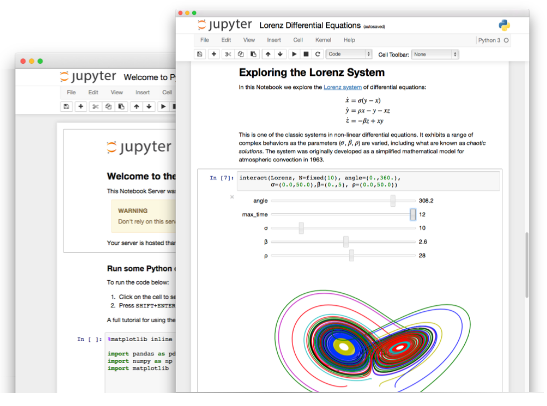
\includegraphics[width=0.85\textwidth]{figures/state-of-the-art/jupyter-notebooks}
  \caption{\Gls{datascience} with Jupyter Notebooks as advertised on their website.}
  \label{fig:jupyter-notebooks}
\end{figure}


\section{Comparison and Summary}

As shown by the presentation of related work, a diverse selection of approaches\index{approach} and tools can be found in this field. Yet, there are also quite some shared aspects to be recognized. For example, basic \gls{gui}s for visual-interactive\index{visual-interactive} schema mapping turned out to develop into pretty similar directions (compare, e.g., the mapping views of \emph{BizTalk} and \emph{Clio} projects as presented in Figure~\ref{fig:biztalk-research-screenshot} and~\ref{fig:clio-screenshot}).

Furthermore, the general \gls{ui} for displaying datasets in this area is spreadsheet-like (see \emph{Potter's Wheel}, \emph{DataWrangler}, \emph{OpenRefine}, and \emph{Talend}).
In addition to that, visual charting aids have started to be incorporated (particularly demonstrated by the more recent time series data related prototype\index{prototype} and commercial tools by \emph{Talend}).
Moreover, modern and innovative approaches\index{approach} are combining classic \emph{\gls{cli}} with scripting, and interactive charting in novel ways (see \emph{Kibana Timelion} and \emph{Jupyter Notebooks}).

Table~\ref{tab:comparison} provides a \textbf{comparison outline} of these projects as well as a preliminary \textbf{requirements list} for our approach.
It should be noted that ``visual interactivity'' is somewhat hard to measure therein, as some approaches\index{approach} lead into quite special directions.

According to these findings there seems to be a need for further research in visual-interactive\index{visual-interactive} aid, for example, via meaningful charts.
Gaps to be filled here are connected to applying interactive \gls{infovis} techniques in order to further improve support of \gls{datawrangling} tasks.
There are approaches\index{approach} already moving into this direction, yet, in particular interactive charting assistance has the potential to substantially facilitate wrangling\index{wrangle} tasks while still needing further research.
As it turns out, visual-interactively\index{visual-interactive} supporting \gls{datawrangling} tasks is currently still in its infancy.
While the general topic of \gls{datawrangling} is not new and quite some research and practice has been done in this field, combining it with \gls{gui}s offering decent \gls{ux} is relatively young.
Especially, incorporating visualization of the to-be-transformed\index{transformation} data and corresponding data transform\index{transformation} operations themselves via meaningful charts is something where further \gls{rnd} is required.

To this end, we are developing a research prototype\index{prototype}, called \emph{\textbf{TempMunger}}, facilitating a visual presentation of the data that enables a better and faster understanding of the data structure and where there is a need for transformation\index{transformation} as well as interactive charts for data manipulation and for giving immediate visual feedback of the transformation\index{transformation}.

\begin{sidewaysfigure}[h]
  \centering
  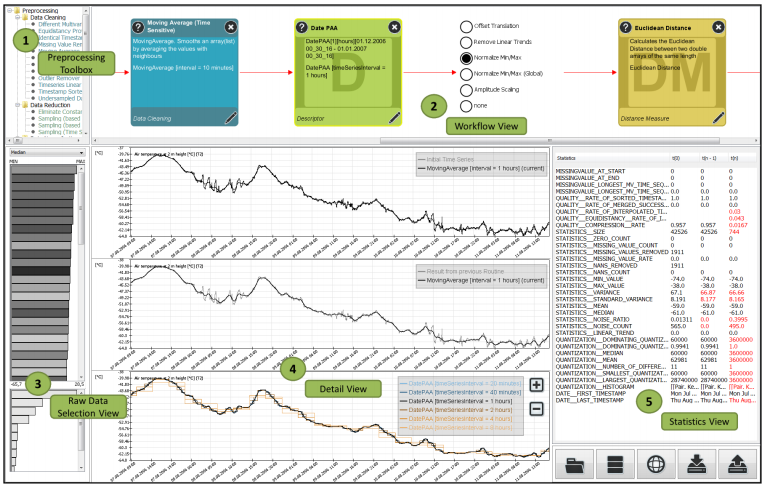
\includegraphics[width=0.95\textwidth]{figures/state-of-the-art/time-series-research}
  \caption{Time series research \gls{ui} with interesting pipeline-based approach (top pane). Various charts (main pane) visualize the data at hand (right pane)~\cite{Bernard2012}.}
  \label{fig:time-series-research-screenshot}
\end{sidewaysfigure}

\begin{sidewaystable}[htb]
  \centering
  \begin{tabular}{|l|c|c|c|c|c|c|c|}
    \hline \textbf{Project} & \textbf{Platform} & \textbf{Domain} & \textbf{GUI Richness} & \textbf{Visual Interactivity} & \textbf{Charts} & \textbf{Time-Oriented} & \textbf{Dashboard}  \\
    \hline
    \hline
    \hline \emph{Potter's Wheel}     & C++, Swing    & Generic         & Medium  & Medium   & No   & No      & No         \\
    \hline \emph{PADS}               & DSL Code, C   & Specific        & N/A     & N/A      & No   & No      & No         \\
    \hline \emph{BizTalk}            & Windows .NET  & Schema Mapping  & Medium  & Medium   & No   & No      & No         \\
    \hline \emph{Clio}               & Java Desktop  & Schema Mapping  & Medium  & Medium   & No   & No      & No         \\
    \hline \emph{Potluck}            & Web           & Semantic Web    & Low     & Medium   & No   & No      & No         \\
    \hline \emph{DataWrangler}       & Web           & Generic         & Medium  & Special  & No   & No      & No         \\
    \hline \emph{OpenRefine}         & Web           & Generic         & Medium  & High     & Yes  & Yes     & No         \\
    \hline \emph{Time Series}        & Unknown       & Specific        & High    & High     & Yes  & Yes     & Partially  \\
    \hline \emph{Talend}             & Eclipse RCP   & Generic         & High    & High     & Yes  & Unknown & Partially  \\
    \hline \emph{Kibana Timelion}    & Web           & Specific        & High    & Special  & Yes  & Yes     & No         \\
    \hline \emph{Jupyter Notebooks}  & Web           & Generic         & High    & Special  & Yes  & Yes     & No         \\
    \hline
    \hline \emph{\textbf{TempMunger}}  & \textbf{Desktop} (Web)  & \textbf{Generic}  & \textbf{High}  & \textbf{High}  & \textbf{Focus}  & \textbf{Highly} & \textbf{Focus}  \\
    \hline
  \end{tabular}
  \caption{Projects comparison serving as a starting point to derive basic requirements.}
  \label{tab:comparison}
\end{sidewaystable}

\begin{sidewaysfigure}[h]
  \centering
  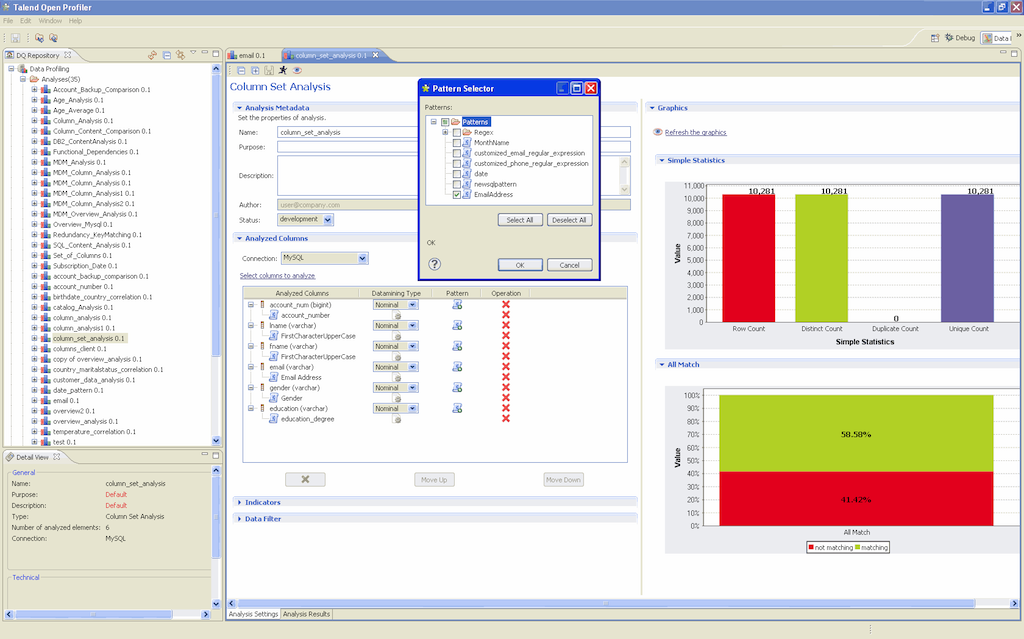
\includegraphics[width=0.95\textwidth]{figures/state-of-the-art/talend-open-studio}
  \caption{Talend Open Studio Data Quality \gls{gui} as an industry-standard solution based on Eclipse \gls{rcp}. Interactively manipulated data (on the left) by transformations (center) is visualized via charting support (right). Screenshot originally taken from product website.}
  \label{fig:talend-open-studio-screenshot}
\end{sidewaysfigure}


\subsection{Our Approach\index{approach}: TempMunger}

Where we are intending to excel with \emph{TempMunger} here is by bringing concepts from both \emph{DataWrangler} and \emph{OpenRefine} together with enhanced visual charting aid as well as our derived requirements (see Section~\ref{sec:requirements-list}) and improved \gls{ux}. The main kind of data to be wrangled\index{wrangle} in particular will be time-oriented\index{time-oriented}. So, focus will be laid on visual-interactive\index{visual-interactive} support of wrangling\index{wrangle} time-oriented\index{time-oriented} data.

More concrete, possible areas of improvement include:

\begin{itemize}
  \item Introduction of modern interaction patterns, like drag \& drop column merging
  \item Visualizing data structures via meaningful charts, presenting transform\index{transformation} suggestions
  \item Directly manipulative interaction with these charts to transform\index{transformation} underlying data
  \item Special focus on supporting time-oriented\index{time-oriented} data with meaningful charts and interactive transformations\index{transformation}
\end{itemize}

Further requirements are derived in Section~\ref{sec:requirements-list} and we expect that more reasonable functionality, features, and constraints will emerge from the iterative \emph{design\index{design} -- implementation -- evaluation} process of the thesis project.

In addition, we are going to tackle the following \gls{datawrangling} challenges as identified by \cite{Kandel2011b}:

\begin{enumerate}
  \item \emph{Diagnosing data problems visually}
  \item \emph{Visualizing ``raw'' data}
  \item \emph{Visual assessment and specification of automated methods}
  \item \emph{Living with dirty data} (visually; i.e., how to display erroneous data best)
\end{enumerate}

While these \gls{infovis} topics are merely directed towards data profiling, we extend upon this by applying it to transformations\index{transformation} connected to \gls{datawrangling}.
\\\\
To sum it up with our main research question, stated once again:

\emph{\textbf{How can we support \gls{datawrangling} with \gls{va} techniques?}}
